\chapter{稳恒电流}\label{chapter-steady-current}

电在生产和生活中的应用越来越广泛,其中许多应用都跟电流有关.电流是在电路中流动的,为了有效地利用和控制电流,需要研究电路的规律.
这一章我们就来学习电路的基本规律和它们的应用.
欧姆定律是分析电路的基础,一定要掌握好,要注意学会用它来分析解决一些简单的电路问题.

\section{电流}
接通电源后,电灯就发光,电炉就发热,电动机就转动,这是因为它们中有了电流.
我们在初中学过,\NoteUnderWave{电荷的定向移动形成电流}.金属导体中的电流是自由电子定向移动形成的.电解液中的电流是正、负离子向相反方向移动形成的.

要形成电流,首先要有能够自由移动的电荷——自由电荷.
金属中的自由电子,电解液中的正、负离子,都是自由电荷.
但是只有自由电荷还不能形成电流.导体中有大量的自由电荷,它们不断地做无规则的热运动,朝任何方向运动的机会都一样.在通常情况下,对导体的任何一个截面来说,在任何一段时间内从截面两侧穿过截面的自由电荷数都相等(图~\ref{fig_B_7-1}),从宏观上看,没有电荷的定向移动,因而也没有电流.
\begin{figure}[htbp]
    \centering
    \begin{minipage}[t]{0.48\linewidth}
    	\centering
    	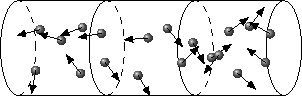
\includegraphics{fig/B/7-1.pdf}
    	\caption{}\label{fig_B_7-1}
    \end{minipage}
   \begin{minipage}[t]{0.48\linewidth}
   		\centering
   		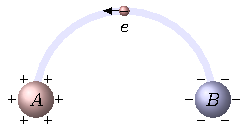
\includegraphics{fig/B/7-2.pdf}
   		\caption{}\label{fig_B_7-2}
   \end{minipage}
\end{figure}

如果把金属导体的一端接在带正电的物体$A$上,另一端接在带负电的物体$B$上(图~\ref{fig_B_7-2}),那么,由于$A$的电势高,$B$的电势低,导体两端有了电势差,导体内就建立了电场.这时,自由电子除了做无规则的热运动外,还要在电场力的作用下做定向移动,即沿着导体从电势低的一端向电势高的一端移动,于是导体中有了电流.但在图~\ref{fig_B_7-2} 所示的情形中不能得到持续的电流.这是因为:随着电子的移动,$A$、$B$上的正、负电荷将逐渐减少,导体两端的电势差也随着减小;当达到静电平衡状态时,导体两端的电势差变为零,导体内的电场强度也变为零,电子不再做定向移动,电流也就消失了.可见,为了使导体中有持续电流,必须设法保持导体两端的电势差.
\NoteUnderWave{导体中存在持续电流的条件,是保持导体两端的电势差}.电源的作用就是保持电路两端的电势差,使电路中有持续的电流.



电流有强弱的不同,电流的强弱用电流强度来表示.\NoteUnderWave{通过导体横截面的电量跟通过这些电量所用的时间的比值,叫做电流强度}.如果时间$t$内通过导体横截面的电量为$q$,那么电流强度
\[I=\frac{q}{t} \]
在国际单位制中,电流强度的单位是\NoteBold{安培},简称安,国际
符号是$\UAA$.
如果在1秒内通过导体横截面的电量是1库仑,导体中的电流强度就是1安培.
常用的电流强度的单位还有毫安($\UImAA$)、微安($\UuAA$).
\[\begin{split}
    1 \UImA &= 10^{-3} \UA\\
    1 \UuA &=10^{-6} \UA
\end{split}\]

导体中的电流既可以是正电荷的移动,也可以是负电荷的移动,还可以是正、负电荷沿相反方向的移动.因为负电荷的移动可看作正电荷沿相反方向的移动,所以为了便于分析问题,习惯上规定正电荷的移动方向为电流的方向.
这样,在金属导体中电流的方向就与自由电子移动的方向相反.在电解液中,电流的方向与正离子移动的方向相同,与负离子移动的方向相反.我们知道,正电荷在电场力的作用下是从电势高处向电势低处移动,所以导体中电流的方向是从电势高的一端流向电势低的一端.
电源上电势高的电极叫正极,电势
低的电极叫负极,所以在电源外部的电路中,电流的方向是从电源的正极流向负极.

电路中,如果电流的方向不随时间而改变,这样的电流叫做\NoteBold{直流电};如果电流的方向和大小都不随时间而改变,这样的电流叫做\NoteBold{稳恒电流}.
这一章我们研究稳恒电流.

\section{欧姆定律}
在导体两端加上电压,导体中就有电流.
导体中电流的强弱跟加在导体两端的电压有什么关系呢?德国物理学家欧姆($1787 \sim 1854$)通过实验研究,对导体中电流与电压的关系
得出了如下的结论:\NoteUnderWave{通过导体的电流跟加在导体两端的电压成正比},即$I\propto U$.通常把这个关系写作
\[\frac{U}{I}=R\]

式中$R$是电压与电流的比值.
实验表明,对同一根导线来说,不管电压和电流的大小怎样变化,比值$R$都是相同的.
对于不同的导线,$R$的数值一般是不同的.这表明,$R$是一个跟导体本身有关的量.
导线的$R$越大,在同一电压下,通过它的电流就越小.可见,比值$R$反映出导线对电流的阻碍作用,我们把它叫做导体的\NoteBold{电阻}.

上面的公式可写成
\[I=\frac{U}{R}\]
这个公式表示\NoteBold{导体中的电流强度跟导体两端的电压成正比,跟导体的电阻成反比}.这就是我们在初中学过的\NoteBold{欧姆定律}.

根据欧姆定律可以规定电阻的单位,电阻的单位是\NoteBold{欧姆},简称欧,国际符号是$\UOA$. 它是这样规定的:如果在某段导线两端加上1伏特电压,通过它的电流强度是1安培,这段导线的电阻就是1欧姆.
\[1 \UO =\frac{1 \UV }{1 \UA} \]

常用的电阻单位还有千欧($\UkOA$)和兆欧($\UMOA$).
\[\begin{split}
    1 \UkO &= 10^{3}\UO\\
    1\UMO &=10^{6}\UO
\end{split}\]

应该注意的是,欧姆定律是在金属导电的基础上总结出来的,对于其他导体是否适用,还要经过实验的检验.实验结果是,除金属外,欧姆定律对电解液导电也适用,但对气体导电就不适用了.

导体中电流跟电压的关系还可以用图线来表示.用横轴表示电压,纵轴表示电流强度,画出的电压--电流图线,叫做导体的伏安特性曲线.在金属导体中,电流强度跟电压成正比,所以伏安特性曲线是通过坐标原点的直线(图~\ref{fig_B_7-3}),直线的斜率等于导体电阻的倒数.导体的电阻越大,伏安特性曲线的斜率越小.同学们可以自己研究一下,图~\ref{fig_B_7-3} 所示的两条伏安曲线,哪一条所代表的电阻大.
\begin{figure}[htbp]
    \centering
    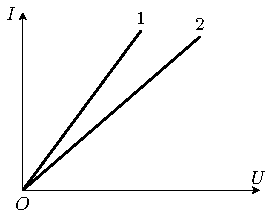
\includegraphics{fig/B/7-3.pdf}
    \caption{金属导体的伏安特性曲线}\label{fig_B_7-3}
\end{figure}


对欧姆定律不适用的导体,它们中的电流与电压不是正
比关系,伏安特性曲线不再是直线.

欧姆定律是电流的基本定律,在研究电路时有很重要的应用.
电流、电压和电阻是电路中的三个基本物理量,根据欧姆定律,知道了其中任意两个量,就可以求出另外一个量.
例如,在保持电压一定的情况下,可以通过改变电阻的办法来控制电路中的电流强度,这在实际中是经常遇到的.


\subsection*{练习一}

\begin{enumerate}
    \item 导线中的电流强度为10安,20秒钟内有多少电子通过导线的横截面?
    \item 手电筒小灯泡上的电压是3伏时,电阻为8.5欧,求通过小灯泡的电流强度.
    \item 人体通过50毫安的电流时,就会引起呼吸器官麻痹.
    如果人体的最小电阻为800欧,求人体的安全工作电压.
    \item 根据上题中所给的数字说明:为什么人体触到220伏的电线时会发生危险,而接触干电池的两极(电压为1.5伏)时却没有感觉?
    \item 电路中有一电阻,测得通过它的电流强度是2毫安时,电阻两端的电压是50毫伏.
    在通过它的电流强度为15毫安时,它两端的电压是多大?
    \item 画出电阻为5欧的导体的伏安特性曲线.
    当导体的电阻增大为10欧时,图线将怎样变化?电阻减小为2.5欧时呢?
\end{enumerate}


\section{电阻定律~~电阻率}
导体的电阻是由导体本身决定的.
那么,决定导体电阻大小的因素究竟有哪些呢?

实验表明,用同一种材料制成的横截面积相等而长度不相等的导线,其电阻跟导线的长度成正比;长度相等而横截面积不相等的导线,其电阻跟导线的横截面积成反比.
\NoteUnderWave{导线的电阻跟它的长度成正比,跟它的横截面积成反比}.这就是\NoteBold{电阻定律},用公式来表示可以写作
\[R=\rho\frac{\ell}{S}\]

式中的比例系数$\rho$跟导体的材料有关系.在一定的温度
下,对同一种材料$\rho$是一个常数,对不同的材料$\rho$的数值不同.
横截面积和长度都相等的不同材料的导线,$\rho$越大的电阻越大,$\rho$越小的电阻越小.可见,$\rho$是一个反映材料导电性好坏的物理量,叫做材料的\NoteBold{电阻率}.

把上面的公式改写作
\[\rho=R\frac{S}{\ell}\]
式中$\ell=1 \Um$,$S=1\Umq$时,$\rho$的数值等于$R$.可见,材料的电阻率在数值上等于这种材料制成的长1$\Um$、横截面积1$\Umq$的导体的电阻.

根据上式,可以确定电阻率$\rho$的单位.
$R$的单位是$\UOA$,$S$的单位是$\UmqA$,$\ell$的单位是$\UmA$,所以$\rho$的单位是欧姆$\cdot$米,简称欧$\cdot$米,国际符号是$\UOmA$.

表~\ref{tab_B_7-1} 列出了几种材料20$\Ucede$时的电阻率.
\begin{table}[htbp]
	\centering
	\caption{}\label{tab_B_7-1}
    \begin{tblr}{cc}
		\toprule
        材料  & $\rho$($\UOmA$)\\
    	\midrule
		银   & $ 1.6\times 10^{-8}$   \\
		铜  & $ 1.7\times 10^{-8}$   \\
		铝  & $ 2.9\times 10^{-8}$   \\
		钨  & $ 5.3\times 10^{-8}$   \\
		铁  & $ 1.0\times 10^{-7}$   \\
		锰铜($85\%\text{铜}+3\%\text{镍}+12\%\text{锰}$)  & $ 4.4\times 10^{-7}$   \\
		康铜($54\%\text{铜}+46\%\text{镍}$) & $ 5.0\times 10^{-7}$   \\
		镍铬合金($67.5\%\text{镍}+15\%\text{铬}+16\%\text{铁}+1.5\%\text{锰}$) & $1.0 \times 10^{-6}$   \\
    \bottomrule
    \end{tblr}
\end{table}
从表~\ref{tab_B_7-1} 可以看出,纯金属的电阻率小,合金的电阻率较大.
金属中银的电阻率最小,但银的价格昂贵,通常很少用银做导线,只在特殊需要时使用.导线一般都用电阻率较小的铜或铝来制作,铝比铜便宜,因此铝导线用得很多.电炉、电阻器的电阻丝一般都用电阻率较大的合金来制作.

各种材料的电阻率都随温度而变化.
金属的电阻率随温度的升高而增大.因此金属导体的电阻也随温度的升高而增大.
利用金属电阻的这种性质可以制作电阻温度计.如果已知导体电阻随温度的变化情况,那么,测出导体的电阻,反过来就可以知道温度.常用的电阻温度计是用铂丝或铜丝制作的.
铂在温度变化时性质稳定,测温范围宽,可靠性好,但是价格昂贵.
铜电阻温度计装置简单,灵敏,在某些特殊条件下,有独特的优点.有些合金,例如康铜和锰铜的电阻率随温度的变化特别小,用这些合金制作的电阻受温度的影响很小,因此常用来作标准电阻.

当温度降低到绝对零度附近时,某些金属、合金和化合物的电阻率会突然减小为零,这种现象叫做\NoteBold{超导现象},处于这种状态的导体叫做\NoteBold{超导体}.超导体的电阻为零,它还具有一系列其他独特的物理性质,有很重要的实用价值.目前,超导体需要的温度很低,使它的应用受到限制.
我国和其他各国现在都在积极进行研究,寻找较高温度下的超导体,探索把超导体应用到实际中去的可能性.

\subsection*{练习二}

\begin{enumerate}
    \item 图~\ref{fig_B_7-4} 是滑动变阻器的结构图.
    涂有绝缘漆的电阻丝密绕在瓷管上,$A$、$B$是它的两个端点,滑动端$P$可在金属杆上移动,它通过金属片与电阻丝接触,把电阻丝和金属杆连接起来.如果把固定端$A$和接线柱$C$接入电路中,当滑动端从$B$向$A$移动时,电路中的电阻就随着变小.
    说明其道理.
    \begin{figure}[htbp]
        \centering
        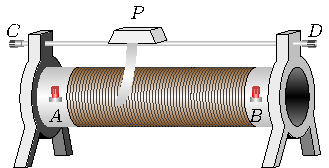
\includegraphics{fig/B/7-4.pdf}
        \caption{滑动变阻器}\label{fig_B_7-4}
    \end{figure}
    \item 一卷铝导线长100米,横截面积为1$\Ummq$,这卷导线的电阻是多大?
    \item 有一段导线,电阻是4欧,把它对折起来作为一条导线用,电阻是多大?如果把它均匀拉长到原来的两倍,电阻又是多大?
    \item 一根做电学实验用的铜导线,长度是60厘米,横截面积是0.5$\Ummq$,它的电阻是多少欧?一根输电用的铜导线,长度是10千米,横截面积是1$\Ucmq$,它的电阻是多少欧?为什么做电学实验时可以不考虑连接用的铜导线的电阻,而对输电线路的导线的电阻则需要考虑?
    \item 一根电阻丝长10米,横截面积是0.2$\Ummq$,两端加上10伏电压时,通过的电流强度是0.2安.这根电阻丝的电阻率是多大?它是用什么材料制作的?
\end{enumerate}

\section{电功和电功率}
我们在初中已经学过电功和电功率,利用上一章所学的知识,我们可以更好地理解这两个重要概念.

在导体两端加上电压,导体内就建立了电场.电场力在推动自由电子定向移动中要做功.
如果导体两端的电压为$U$,通过导体横截面的电量为$q$,那么,从上一章讲的可知,电场力所做的功$W=qU$.由于$q=It$,所以,
\[W=UIt\]
上式中$W$、$U$、$I$、$t$的单位应分别用焦耳、伏特、安培、秒.

电场力做的功常常说成是电流做的功,简称电功.所以,\NoteUnderWave{电流在一段电路上所做的功,跟这段电路两端的电压、电路中的电流强度和通电时间成正比}.

电场力做功时,正电荷从导体电势高的一端移向电势低的一端,电势能减少.这时减少的电能转化为其他形式的能.可见,电流通过用电器做功的过程,实际上是电能转化为其他形式的能的过程.例如,电流通过电炉做功,电能转化为内能;电流通过电动机做功,电能转化为机械能;电流通过电解槽做功,电能转化为化学能.电流做了多少功,就有多少电能转化为其他形式的能.

电流所做的功跟完成这些功所用的时间的比值叫做电功率.
用P表示电功率,那么
\[P=\frac{W}{t}=UI\]
上式中$P$、$U$、$I$的单位应分别用瓦特、伏特、安培.

可见,\NoteUnderWave{一段电路上的电功率,跟这段电路两端的电压和电路中的电流强度成正比}.

为了使用电器安全正常地工作,制造厂对用电器的电功率和工作电压都有规定的数值,并且标明在用电器上,叫做用
电器的额定功率和额定电压.给用电器加上额定电压,用电器正常工作时的功率就是额定功率.
例如,标有“220V,40W”的灯泡,接在220伏的线路中,灯泡正常发光,它的功率为40瓦.
这时通过灯泡的额定电流为$(40/220) \UA =0.18 \UA $.
如果接在高于220伏的线路中,通过灯泡的电流增大,它消耗的实际功率也增大,灯泡有烧坏的危险;如果接在低于220伏的线路中,通过灯泡的电流减小,它消耗的实际功率也减小,灯泡将变得昏暗不亮.可见,加在用电器上的电压改变时,通过它的电流也改变,它的实际功率也随着改变.

\section{焦耳定律}
\subsection{焦耳定律}


电流通过导体时要产生热,使导体的内能增加,温度升高,这就是电流的热效应.
英国物理学家焦耳用实验研究了这个问题,指出:
\NoteUnderWave{电流通过导体产生的热量,跟电流强度的平方、导体的电阻和通电时间成正比}.
这就是我们在初中学过的\NoteBold{焦耳定律}.如果热量$Q$的单位用焦耳,电流强度$I$的单位用安培,电阻$R$的单位用欧姆,时间$t$的单位用秒,焦耳定律可以写成如下的公式
\[Q=I^2Rt\]

电流的热效应在生产和生活中有许多实际应用.
电灯、电炉、电烙铁、电烘箱等都是利用电流的热效应制作的.但是,电流的热效应在有些地方是有害的.
例如,电流通过输电导线、电动机的线圈、电视机中的零件时都要产生热,这不仅
白白消耗电能,而且如果产生的热量使温度升高过多,还会使它们损坏,因此实际中要注意通风散热.

\subsection{电功和电热的关系} 

电流通过电路时要做功,同时,一般电路都是有电阻的,因此电流通过电路时也要产生热.那么,电流做的功跟它产生的热之间又有什么关系呢?

如果电路中只含有电灯、电炉等纯电阻性元件,即所谓纯电阻电路,由于这时电路两端的电压$U=IR$,因此$UIt=I^2Rt$.这就是说,电流所做的功$UIt$跟产生的热量$I^2Rt$是相等的.在这种情况下,电能完全转化为内能.这时电功的公式也可以写成
\[W=I^2Rt=\frac{U^2}{R}t\]

如果电路中还包含有电动机、电解槽等用电器,即电路不
是纯电阻性的,那么,电能除部分转化为内能外,还要转化为机械能、化学能等.
这时电功仍然等于$UIt$,产生的热量仍然等于$I^2Rt$,但电流所做的功已不再等于产生的热量,而是大于这个热量;加在电路两端的电压$U$也不再等于$IR$,而是大于$IR$了.在这种情况下,就不能再用$I^2Rt$或$\dfrac{U^2}{R}t$来计算电功.

例如,一台电动机,额定电压是110伏,正常工作时通过的电流是50安.每秒钟内电流做的功是$UIt=5.5\times10^3\UJ $.电动机线圈的电阻只有0.40欧,每秒钟产生的热量是$I^2Rt=1.0\times10^3 \UJ $.电功比电热大很多,大部分电能变为机械能了.

总之,只有在纯电阻电路里,电功才等于电热;在非纯电阻电路里,要注意电功和电热的区别.

\subsection*{练习三}
\begin{enumerate}
    \item 额定电压相同、额定功率不同的两只灯泡,哪个的额定电流大?哪个的电阻大?
    \item 用户保险盒中安装的保险丝允许通过的最大电流一般都不大(几个安培),如果在电路中接入功率在1000瓦以上的用电器,如电炉等,就会把保险丝烧断,这是为什么?
    \item 日常使用的电功单位是“度”,等于功率为1千瓦的电流在1小时内做的功,又叫千瓦时.
    1度等于多少焦?
    \item 有一个1千瓦、220伏的电炉,正常工作时电流是多少?如果不考虑温度对电阻的影响,把它接在110伏的电压上,它的功率将是多少?
    \item 输电线的电阻共计1.0欧,输送的电功率是100千瓦.
    用400伏的低压送电,输电线上发热损失的功率是多少千瓦?改用1万伏的高压送电呢?
    \item 用功率为2千瓦的电炉把2千克的水从20$\Ucede$加热到100$\Ucede$,如果电炉的效率为30\%,需要多少时间?水的比热为$4.2\times10^3 \UJkgcede$.
\end{enumerate}

\section{串联电路}
把导体一个接一个地依次连接起来,就组成串联电路.
图~\ref{fig_B_7-5} 是由三个电阻$R_1$、$R_2$、$R_3$组成的串联电路.在串联电路中,电流沿着一条通路依次流过各个电阻,没有分岔,因此\NoteUnderWave{流过串联电路各电阻的电流强度相等}.
\begin{figure}[htbp]
    \centering
    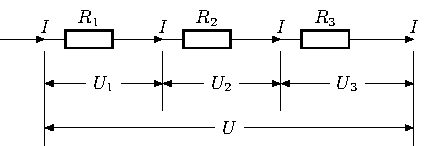
\includegraphics{fig/B/7-5.pdf}
    \caption{串联电路}\label{fig_B_7-5}
\end{figure}	

电流通过串联电路各电阻时,沿电流方向每通过一个电阻,电势要降低一定的数值,因此电阻两端的电压又叫做电势降落.电流在各电阻上的电势降落之和就是串联电路两端的
电势降落,即总电压(图~\ref{fig_B_7-6}).\NoteUnderWave{串联电路两端的总电压等于各部分电路两端的电压之和}.在图~\ref{fig_B_7-5} 中就是
\[U=U_1+U_2+U_3\]
\begin{figure}[htbp]
    \centering
    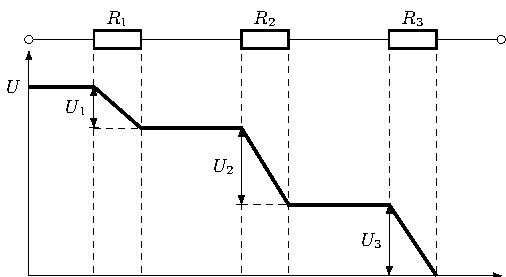
\includegraphics{fig/B/7-6.pdf}
    \caption{}\label{fig_B_7-6}
\end{figure}


上面讲的是串联电路中电流、电压的基本特点.
利用欧姆定律和这些基本特点来研究串联电路的总电阻、电压分配、功率分配等,还可以得出一些特殊的关系和结论,这些结论对于分析、计算电路很有用处.下面我们就分别来进行研究.

\subsection{串联电路的总电阻} 
串联电路中的几个电阻可以用一个电阻来代替,把这个电阻接入串联电路两端时,在相同的
总电压下,通过电路中的电流强度跟原来的相等,也就是说,这个电阻在电路中的作用效果跟原来的几个串联电阻一样.这样的电阻叫做串联电路的等效电阻,也叫串联电路的总电阻.如果用R表示总电阻,那么,根据欧姆定律,在图~\ref{fig_B_7-5} 中,
\[U=IR,\qquad  U_1=IR_1,\qquad U_2=IR_2,\qquad U_3=IR_3\]
把上面的公式代入$U=U_1+U_2+U_3$中,整理后可得
\[R=R_1+R_2+R_3\]

如果串联电路中有$n$个电阻,同理可以推出
\[R=R_1+R_2+R_3+\cdots+R_n\]

这就是说,\NoteUnderWave{串联电路的总电阻,等于各导体的电阻之和}.

利用串联电路电阻的这个规律,在需要增大电路的电阻时,我们就可以在电路中串联上一个或几个电阻.

\subsection{串联电路的电压分配}
串联电路两端的总电压等于
各串联电阻上的电压之和,那么各电阻上的电压跟电阻有什么关系呢?在串联电路中,由于
\[U=IR,\;  U_1=IR_1,\; U_2=IR_2,\; U_3=IR_3,\cdots, U_n=IR_n\]
所以,
\[\frac{U_1}{R_1}=\frac{U_2}{R_2}=\frac{U_3}{R_3}=\cdots=\frac{U_n}{R_n}=I \]
这表明,\NoteUnderWave{串联电路中各个电阻两端的电压跟它的阻值成正比}.阻值越大的电阻,两端的电压也越大.

串联电路的每个电阻都分担了一部分电压.在电路中的电压超过用电器额定电压的情况下,可以在电路中串联上电阻,以分去一部分电压,使用电器得到所需的电压.
串联电阻的这种作用叫做分压作用,起分压作用的电阻叫做分压电阻.

在电学实验中,常用滑动变阻器接成分压器电路来调节
用电器或工作电路所需的电压的大小.滑动变阻器用作分压器时的电路如图~\ref{fig_B_7-7} 所示,变阻器的两个固定端连接在电源$ab$上,其中一个固定端和滑动端$P$跟用电器或工作电路的两端相连.改变滑动端在两个固定端间的位置,输出电压$U_{cd}$就可以在$0 \sim U$之间变化.
\begin{figure}[htbp]
	\centering
	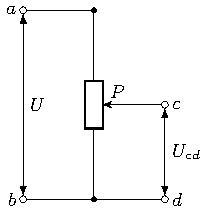
\includegraphics{fig/B/7-7.pdf}
	\caption{分压器电路}\label{fig_B_7-7}
\end{figure}

\subsection{串联电路的功率分配} 串联电路中某个电阻$R_k$消耗的功率$P_k=U_kI$,而$U_k=IR_k$,所以$P_k=I^2R_k$.因此各个电阻消耗的功率分别是
\[P_1=I^2R_1,\; P_2=I^2R_2,\; P_3=I^2R_3,\cdots, P_n=I^2R_n\]
所以
\[\frac{P_1}{R_1}=\frac{P_2}{R_2}=\frac{P_3}{R_3}=\cdots=\frac{P_n}{R_n}=I^2 \]

这就是说,\NoteUnderWave{串联电路中各个电阻消耗的功率跟它的阻值成正比}.在串联电路中,阻值越大的电阻,消耗的功率越大.

整个串联电路消耗的总功率
\[P=UI=I^2R_1 +I^2R_2+I^2R_3+\cdots+I^2R_n
\]
所以
\[P=P_1+P_2+P_3+\cdots +P_n\]

可见,串联电路中消耗的总功率等于各部分电路消耗的功率之和.



\begin{example}
    图~\ref{fig_B_7-8} 是实际中常用的一种分压电路,用分压电阻$R_2$分去一部分电压,使$R_1$上得到所需的电压$U_1$.如果加在该电路上的电压$U=50$伏,电阻$R_1=1$千欧,要使$U_1=
    5$伏,分压电阻$R_2$的阻值应为多大?
\end{example}

\begin{figure}[htbp]
	\centering
	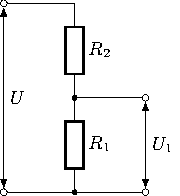
\includegraphics{fig/B/7-8.pdf}
	\caption{}\label{fig_B_7-8}
\end{figure}

\begin{solution}
    设$R_2$上的电压为$U_2$,电路中的电流强度为$I$.根据欧姆定律,$U_2=IR_2$,可以求得
    \[R_2=\frac{U_2}{I}\]

因为串联电路两端的电压等于各部分电路电压之和,所
以在图~\ref{fig_B_7-8} 中$U=U_1+U_2$.由此可求出$R_2$上的电压
\[U_2=U-U_1=(50-5) \UV =45 \UV\]

从$U_1=IR_1$,可得
\[ I=\frac{U_1}{R_1}=\frac{5}{1000} \UA =5\times10^{-3} \UA\]

将求得的$I$、$U_2$代入$R_2$中,即得
\[R_2=\frac{U_2}{I}=\frac{45}{5\times10^{-3}} \UO =9\UkO\]

$R_2$也可以利用串联电路的电压分配公式求得,因为
\[\frac{U_1}{R_1}=\frac{U_2}{R_2}\]
由此可得
\[R_2=\frac{U_2R_1}{U_1}=\frac{45/1000}{5}\UO=9\UkO \]
\end{solution}

显然,后一种解法简便得多.
可见,掌握了串联电路的特殊规律,可以使电路的分析、计算得到简化.

\subsection*{练习四}
\begin{enumerate}
    \item 电炉和导线是串联的,把它们接入电源后,导线和电炉丝中通过的电流强度是否一样?为什么这时电炉丝热得发红,导线并不热?
    \item 某同学要为游艺晚会准备一棵装有彩色电灯的小松树,如果所用的每只灯泡的额定电压是8伏,用220伏的市电做电源,那么需要将多少只灯泡串联在一起才能接在电源上?
    \item 一个量程为150伏的电压表,内阻为20千欧,把它与一高电阻串联后接在110伏的电路上,电压表的读数是5伏.求高电阻的阻值是多少?(这是测量高电阻的一种方法)
    \item 直流电动机线圈的电阻很小,所以起动时的电流很大,这对电动机本身和接在同一电源上的其他用电器都产生不良的后果.为了减小电动机起动时的电流,需要给电动机串联一个起动电阻$R$,如图~\ref{fig_B_7-9} 所示.
    电动机起动后再将$R$逐渐减小.
    如果电源电压$U=220 \UV$,电动机的线圈电阻$r_0=2\UO$,那么,
    \begin{enumerate}
        \item 不串联电阻$R$时的起动电流是多大?
        \item 为了使起动电流减小为20安,起动电阻应为多大?
    \end{enumerate}
    
    \begin{figure}[htbp]
    	\centering
    	\begin{minipage}[t]{0.48\textwidth}
    		\centering
    		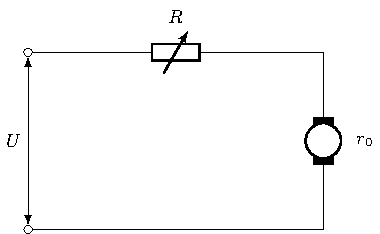
\includegraphics{fig/B/7-9.pdf}
    		\caption{}\label{fig_B_7-9}
    	\end{minipage}
    	\begin{minipage}[t]{0.48\textwidth}
    		\centering
    		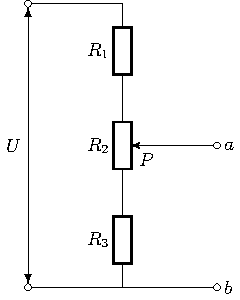
\includegraphics{fig/B/7-10.pdf}
    		\caption{}\label{fig_B_7-10}
    	\end{minipage}
    \end{figure}
    
    \item 图~\ref{fig_B_7-10} 是一个变阻器分压电路.
    如果电压$U=12\UV$,$R_1=350\UO$,$R_2=270\UO$,$R_3=550\UO$,那么,滑动端$P$从$R_2$下端向上移动时,$a$、$b$间的电压将怎样变化?当$P$在$R_2$最下端和最上端时,$a$、$b$间的电压各是多少?	
\end{enumerate}


\section{并联电路}


把几个导体并列地连接起来,就组成了并联电路.同一电路上的各个用电器,通常都是采用并联接法.图~\ref{fig_B_7-11} 是三个电阻$R_1$、$R_2$、$R_3$组成的并联电路.

\begin{figure}[htbp]
	\centering
	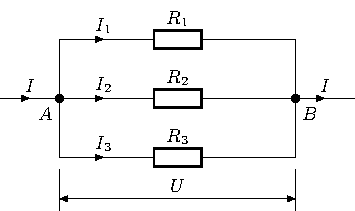
\includegraphics{fig/B/7-11.pdf}
	\caption{并联电路}\label{fig_B_7-11}
\end{figure}


从图~\ref{fig_B_7-11} 中可以看出,三个并联电阻的首端都连接在一点$A$上,尾端都连接在一点$B$上,所以每个电阻两端的电压都等于$A$、$B$两点间的电压.由此可知,\NoteUnderWave{并联电路中各支路两端的电压相等}.

电流通过并联电路时,总电流分成几条支路.在初中我们通过实验已经知道,并联电路中各支路的电流强度之和等于总电流强度.
在图~\ref{fig_B_7-11} 中,流入$A$点的电流$I$等于从该点流出的电流$I_1$、$I_2$、$I_3$之和,即
\[I=I_1+I_2+I_3\]
所以,\NoteUnderWave{并联电路中的总电流强度等于各支路电流强度之和}.


以上是并联电路中电压、电流的基本特点.
应用欧姆定律和这些基本特点来研究并联电路的总电阻、电流分配和功率分配,也可以得出一些有用的关系式和结论.

\subsection{并联电路的总电阻}
并联电路的几个电阻也可以用
一个电阻来代替,把这个电阻接在并联电路的两端时,在相同
的电压下,电路中的总电流保持变,这样的电阻叫做并联电路的等效电阻,也叫做并联电路的总电阻.用$R$代表并联电路的总电阻,根据欧姆定律,在图~\ref{fig_B_7-11} 中,
\[I=\frac{U}{R};\quad I_1=\frac{U_1}{R_1};\quad I_2=\frac{U_2}{R_2};\quad I_3=\frac{U_3}{R_3}\]
将上面各式代入$I=I_1+I_2+I_3$中,整理后可得
\[\frac{1}{R}=\frac{1}{R_1}+\frac{1}{R_2}+\frac{1}{R_3} \]
如果电路中有$n$个导体并联,同理可以推出
\[\frac{1}{R}=\frac{1}{R_1}+\frac{1}{R_2}+\frac{1}{R_3}+\cdots+\frac{1}{R_n} \]
这就是说,\NoteUnderWave{并联电路总电阻的倒数,等于各个导体的电阻倒数之和}.所以,并联电路的总电阻比每一个电阻都小.
利用这个规律,在需要减小某一部分电路的电阻时,只要在这部分电路中并联上一个适当的电阻就行了.

\subsection{并联电路的电流分配}
并联电路中各支路两端的电压相等,根据欧姆定律,在并联电路中,
\[I_1R_1=I_2R_2=I_3R_3=\cdots=I_nR_n=U \]

这就是说,\NoteUnderWave{并联电路中通过各导体的电流强度跟它的电阻成反比}.电阻越小的导体,通过的电流强度越大.

在电路中并联一个电阻$R$,电流就多了一条通路,可以分去电路中的一部分电流(图~\ref{fig_B_7-12}).在电路中电流强度超过某个元件所能允许的电流强度的情况下,给它并联上一个适当的电阻,就可以使通过元件的电流减小到允许的数值.并联电
阻的这种作用叫做分流作用,起分流作用的电阻叫做分流电阻.
\begin{figure}[htbp]
    \centering
    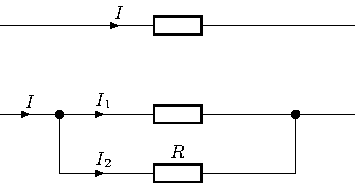
\includegraphics{fig/B/7-12.pdf}
    \caption{并联电阻$R$的分流作用}\label{fig_B_7-12}
\end{figure}

\subsection{并联电路的功率分配}
并联电路中某个电阻$R_k$消耗的功率$P_k=UI_k$,而$I_k=U/R_k$,所以$P_k=U^2/R_k$.因此各个电阻消耗的功率分别是
\[ P_1=\frac{U^2}{R_1},\;  P_2=\frac{U^2}{R_2},\; \cdots  P_n=\frac{U^2}{R_n} \]
所以,
\[P_1R_1=P_2R_2=\cdots=P_nR_n=U^2 \]
这就是说,\NoteUnderWave{并联电路中各个电阻消耗的功率跟它的阻值成反比}.在并联电路中,阻值越大的电阻,消耗的功率越少.

整个并联电路消耗的总功率
\[P=UI=U (I_1+I_2+I_3+\cdots+I_n) \]
所以
\[P=P_1+P_2+P_3+\cdots+P_n\]
即消耗的总功率等于各支路上消耗的功率之和.

\subsection*{练习五}
\begin{enumerate}
    \item 电路中需要一个阻值为15千欧的电阻,现在手边只有几只10千欧的电阻,怎样才能组成一个15千欧的电阻?
    \item 在图~\ref{fig_B_7-13} 所示的电路中,$R_1=10\UO$,$R_2=30\UO$,$U=6\UV$.
    电键$K$合上前后,
    \begin{enumerate}
        \item 电路中的总电阻各是多少?
        \item 通过$R_1$、$R_2$的电流强度各是多少?
        \item $R_1$、$R_2$上消耗的功率各是多少?
    \end{enumerate}
    \begin{figure}[htbp]
    	\centering
    	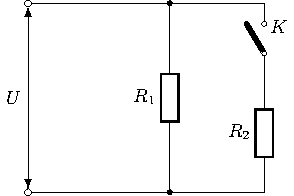
\includegraphics{fig/B/7-13.pdf}
    	\caption{}\label{fig_B_7-13}
    \end{figure}
    \item 在图~\ref{fig_B_7-14} 所示的电路中,要使通过$R_1$的电流强度不超过5毫安,分流电阻$R_2$应为多大?
    \begin{figure}[htbp]
    	\centering
    	\begin{minipage}[t]{0.48\textwidth}
    		\centering
    		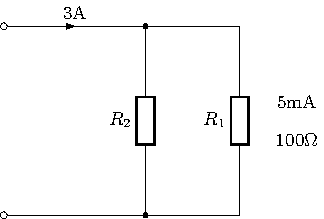
\includegraphics{fig/B/7-14.pdf}
    		\caption{}\label{fig_B_7-14}
    	\end{minipage}
    	\begin{minipage}[t]{0.48\textwidth}
    		\centering
    		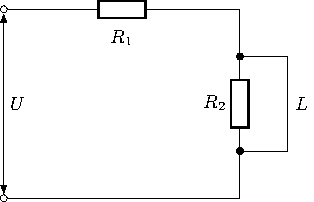
\includegraphics{fig/B/7-15.pdf}
    		\caption{}\label{fig_B_7-15}
    	\end{minipage}
    \end{figure}
    \item 在图~\ref{fig_B_7-15} 所示的电路中,$L$是跟$R_2$并联的一条导线,下列说法哪些是正确的?
    \begin{enumerate}
        \item 通过$R_1$、$R_2$的电流强度$I$相等:
        \[I=\frac{U}{R_1+R_2} \]
        \item $R_1$上的电压$U_1=R_1I$,$R_2$上的电压$U_2=R_2I$,导线$L$中的电流为零.
        \item $R_1$上的电压$U_1=U$,$R_2$上的电压为零.
        \item $R_1$中的电流强度$I_1=U/R_1$,导线$L$中的电流强度等于$I_1$;$R_2$中的电流强度为零.
\item $R_2$去掉后,电路中的电阻和电流强度不发生变化.
    \end{enumerate}
\end{enumerate}



\section{分压和分流在伏特表和安培表中的应用}
作为应用串联电阻进行分压和并联电阻进行分流的实例,我们来研究一下它们在伏特表和安培表中的应用.

常用的安培表和伏特表都是由电流表改装的.
关于电流表的构造和工作原理我们将在以后学习,这里先简单说明一下.在电流表里有一个线圈,当线圈中有电流通过时,在磁场力的作用下线圈就带着指针一起偏转,通过线圈的电流越大,指针的偏角就越大,因此,根据指针的偏角就可以知道电流的大小.
这样,如果在刻度盘上标出电流值就可以测定电流了.我们知道,通过电流表的电流跟加在电流表两端的电压成正比,因此,指针的偏角越大,表示加在电流表两端的电压越大,这样,如果在刻度盘上直接标出电压值,就可以测定电压了.

电流表的线圈是用很细的铜丝绕成的,允许通过的最大电流很小,一般不超过几十微安到几毫安,这个电流用$I_g$表示.
线圈的电阻一般为几百到几千欧,叫做电流表的内阻,用$R_g$表示.每个电流表都有它的$R_g$值和$I_g$值.当通过它的电流为$I_g$时,它的指针偏转到最大刻度处,所以$I_g$叫满度电流.如果电流超过满度电流,不但指针指示不出数值,电流表还可能烧毁.

\subsection{伏特表}


电流表虽然能够用来测电压,但是由于电流表能够承担的电压$I_gR_g$很小,所以不能直接用电流表来测较大的电压.如果被测电压$U$大于$I_gR_g$,通过电流表的电流将超过$I_g$可能把电流表烧毁.如果给电流表串联一个电阻,分担一部分电压,就可以用来测较大的电压了.加了串联电阻并
在刻度盘上标出伏特值,就把电流表改装成了伏特表(图~\ref{fig_B_7-16}).伏特表刻度盘上标出的伏特值,不是表示加在电流表上的电压,而是直接表示加在伏特表上的电压.
\begin{figure}[htbp]
    \centering
    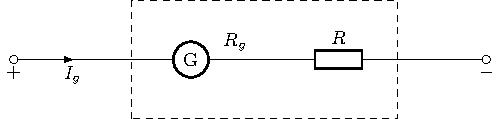
\includegraphics{fig/B/7-16.pdf}
    \caption{}\label{fig_B_7-16}
\end{figure}

让我们用一个具体例子来说明如何改装.
假设有一个电流表,内阻$R_g$是1000欧,满度电流$I_g$是100微安.
要把它改装成量程是3伏的伏特表,应该串联多大的电阻呢?

电流表指针偏转到满刻度时,它两端的电压$U_g=I_gR_g=0.1\UV$,这是它能承担的最大电压.
现在要让它测量最大为
3伏的电压,即指针偏转到满刻度时伏特表两端的电压为3伏,分压电阻$R$就必须分担2.9伏的电压.串联电路中电压跟电阻成正比,
\[\frac{U_g}{R_g}=\frac{U}{R}\]
由此可以求出
\[R=\frac{U_R}{U_g}R_g=\frac{2.9}{0.1}\times 1000\UO=29{\rm k}\UO\]
可见,串联29千欧的分压电阻后,就可以把这个电流表改装成量程为3伏的伏特表.

从上面的计算可以看出,把电流表改装成伏特表,需要给电流表串联一个阻值大的电阻.改装后的伏特表量程越大,需要分去的电压也越大,串联的分压电阻就要越大.

\subsection{安培表}


电流表能够测量的电流不超过毫安级.为了测量几个安培甚至更大的电流,可以给它并联一个分流电阻,分掉一部分电流.这样,在测量大电流时通过电流表的电流也不致超过满度电流$I_g$.并联了分流电阻并在刻度盘上标出安培值,电流表就改装成了安培表(图~\ref{fig_B_7-17}).安培表刻度盘上标出的安培值,不是表示通过电流表的电流,而是直接表示通过安培表的电流.
\begin{figure}[htbp]
    \centering
    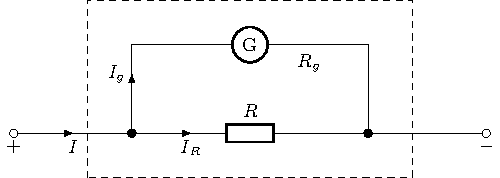
\includegraphics{fig/B/7-17.pdf}
    \caption{}\label{fig_B_7-17}
\end{figure}

例如,电阻$R_g$是1000欧、满度电流$I_g$是100微安的电流表,要改装成量程为1安的安培表,我们很容易计算出应该并联多大的分流电阻.

电流表允许通过的最大电流是$100 \UuA=0.0001 \UA $,在测量1安的电流时,分流电阻R上通过的电流应该是$I_R=0.9999 \UA $.
由于并联电路中电流强度跟电阻成反比,$I_gR_g=I_R R$.所以,
\[R=\frac{I_g}{I_R}R_g=\frac{0.0001}{0.9999}\times 1000\UO=0.1\UO\]
可见,并联0.1欧的分流电阻后,就可以把这个电流表改装成量程为1安的安培表.
把电流表改装成安培表,需要给它并联一个阻值小的电阻,改装后的安培表量程越大,需要分去的电流也越大,并联的分流电阻就要越小.


\subsection*{练习六}

\begin{enumerate}
    \item \label{exe_B-7-6-1}
    有一个电流表,内阻为100欧,满度电流为3毫安,要把它改装成量程为3安的安培表,需并联多大的分流电阻?要把它改装为6伏的伏特表,需串联多大的电阻?
    \item \label{exe_B-7-6-2}
    电流表的内阻为$R_g$,满度电流为$I_g$.试证明:
     \begin{enumerate}
         \item 要把它改装成量程为$U=nI_gR_g$的伏特表,串联电阻的阻值应为
         \[R_{\text{串}}=(n-1)R_g\]
         \item 要把它改装成量程为$I=nI_g$的安培表,并联电阻的阻值应为
         \[R_{\text{并}}=R_g/(n-1)\]
     \end{enumerate}
     \item 在第 \ref{exe_B-7-6-1} 题中,改装后的安培表的量程比电流表原来的电流量程扩大的倍数$n$是多少?改装后的伏特表比电流表原来的电压量程扩大的倍数$n$又是多少?利用第 \ref{exe_B-7-6-2} 题中推出的两个公式,重新计算第 \ref{exe_B-7-6-1} 题中的并联电阻和串联电阻,比较两次计算的结果是否相同.
     \item 有一安培表,内阻为0.03欧,量程为3安.
     测量电阻$R$中的电流强度时,本应与$R$串联,如果不注意,错把安培表与$R$并联了(图~\ref{fig_B_7-18}),将会产生什么后果?假设$R$两端的电压为3伏.
\end{enumerate}
\begin{figure}[htbp]
    \centering
    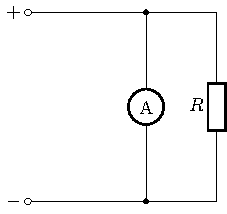
\includegraphics{fig/B/7-18.pdf}
    \caption{}\label{fig_B_7-18}
\end{figure}

\section{电路的分析和计算}

实际应用的电路大多是既包含并联电路又包含串联电路的混联电路.
运用前面讲过的串联电路和并联电路的知识就可以对混联电路进行分析和计算.
下面举两个例子来说明混联电路的实际意义和它的分析计算方法.

\begin{example}
    线路电压为220伏,每根输电导线的电阻$r=1 \UO $,电路中并联了100盏“$220 \UV$,$40 \UW$”的电灯.求:
    \begin{enumerate}
        \item 只打开其中的10盏灯时每盏灯的电压和功率;
        \item 100盏灯全部打开时每盏灯的电压和功率.
    \end{enumerate}
\end{example}

\begin{solution}
    根据题意,100盏电灯是并联的,电灯与输电导线是串联的,电路如图~\ref{fig_B_7-19} 所示,其中$r$是每根输电导线的电阻.从图上可以看出,电灯的电压等于线路电压减去输电导线上的电压.求出并联电灯的电阻$R_{\text{并}}$、电路的总电阻$R_{\text{总}}$,算出电路中的总电流强度,就可以求出输电导线上的电压,从而可以求得电灯的电压和功率.
    \begin{figure}[htbp]
        \centering
        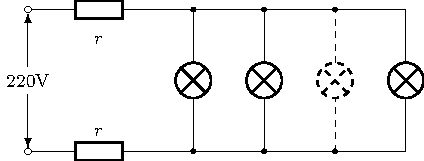
\includegraphics{fig/B/7-19.pdf}
        \caption{}\label{fig_B_7-19}
    \end{figure}

\begin{enumerate}
\item
只打开10盏电灯的时候:

每盏电灯的电阻
\[R=\frac{U^2}{P}=\frac{220^2}{40}\UO=1210\UO \]
10盏电灯并联的电阻
\[R_{\text{并}}=\frac{R}{10}=121\UO\]
电路中的总电阻
\[R_{\text{总}}=R_{\text{并}}+2r=(121+2)\UO=123\UO \]
电路中的总电流强度
\[I=\frac{U}{R_{\text{总}}}=\frac{220}{123} \UA =1.8\UA\]
两根输电导线上的电压
\[2U_r=2Ir =2\times1.8\times 1 \UV=3.6\UV\]
电灯的电压
\[U_L=U-2U_r=(220-3.6)\UV=216.4\UV\]
每盏电灯的功率
\[P=\frac{U^2_L}{R}=\frac{216^2}{1210} \UW=39\UW\]

\item 
100盏电灯全部打开的时候:100盏电灯并联的电阻
\[R_{\text{并}}=\frac{R}{100}=12.1\UO\]
电路中的总电阻
\[R_{\text{总}}=R_{\text{并}}+2r=(12.1+2) \UO =14.1\UO \]
电路中的总电流强度
\[I=\frac{U}{R_{\text{总}}}=\frac{220}{14.1} \UA=16\UA\]
两根输电导线上的电压
\[2U_r=2Ir =2\times16\times 1 \UV=32\UV\]
电灯的电压
\[U_L=U-2U_r=(220-32) \UV=188\UV\]
每盏电灯的功率
\[P=\frac{U^2_L}{R}=\frac{188^2}{1210} \UW =29\UW\]
\end{enumerate}

\end{solution}

从这道例题可以看出,100盏电灯全部打开时比只打开10盏时加在电灯上的电压减小了,每盏灯上消耗的功率也减小了.一般说来,电路里并联的用电器越多,并联部分的电阻就越小,在总电压不变的条件下,电路里的总电流就越大,因此输电线上的电压就越大.这样,加在用电器上的电压就越小,每个用电器消耗的功率也越小.我们在晚上七、八点钟开灯,那时大家都用电灯照明,电灯比深夜时暗些,就是这个缘故.

\begin{example}
图~\ref{fig_B_7-20a} 是一个分压器电路,由两个10千欧的电阻串联而成.线路两端电压为50伏时,$a$、$b$间的电压应为25伏.用内阻为25千欧的伏特表$V_1$测量$a$、$b$间的电压时,伏特表的读数不到21伏;改用内阻为500千欧的伏特表$V_2$测量时,伏特表的读数接近25伏.试分析其原因.
\end{example}
\begin{figure}[htbp]
    \centering
    \begin{subfigure}{0.3\linewidth}
        \centering
        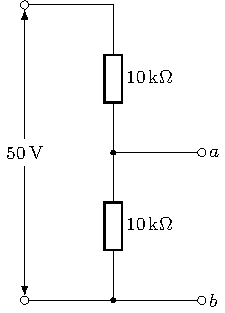
\includegraphics{fig/B/7-20a.pdf}
        \caption{}\label{fig_B_7-20a}
    \end{subfigure}
    \hfil
    \begin{subfigure}{0.3\linewidth}
        \centering
        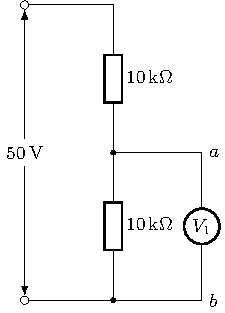
\includegraphics{fig/B/7-20b.pdf}
        \caption{}\label{fig_B_7-20b}
    \end{subfigure}
    \hfil
    \begin{subfigure}{0.3\linewidth}
        \centering
        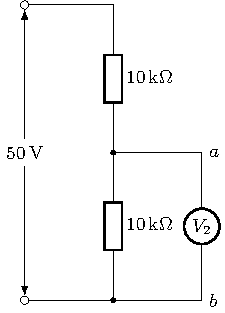
\includegraphics{fig/B/7-20c.pdf}
        \caption{}\label{fig_B_7-20c}
    \end{subfigure}
    \caption{}\label{fig_B_7-20}
\end{figure}

\begin{solution}
    伏特表未接入电路时,$a$、$b$间的电压$U_{ab}=25\UV$(图~\ref{fig_B_7-20a}).
    伏特表接入电路后,伏特表与下面的10千欧电阻形成并联(图~\ref{fig_B_7-20b} 和 \ref{fig_B_7-20c}),整个电路变为混联电路.由于$a$、$b$间的电阻发生变化,所以电压也发生变化.这就是为什么伏特表测得的结果不是25伏的原因.
\begin{enumerate}
\item
用内阻为25千欧的伏特表$V_1$测量时(图~\ref{fig_B_7-20b}),$a$、$b$间的并联电阻
\[R_{\text{并}}=\frac{25\times 10}{25+10} \UkO=7.1\UkO\]
电路中的总电阻
\[R_{\text{总}}=(10+7.1) \UkO=17.1\UkO \]
电路中的电流强度
\[I=\frac{U}{R_{\text{总}}}=\frac{50}{17.1\times 10^4} \UA=2.9\times 10^{-3} \UA \]
$a$、$b$间的电压,即伏特表$V_1$测得的电压
\[U_{ab}=IR_{\text{并}}=2.9\times10^{-3}\times7.1\times10^3 \UV=20.6\UV\]

\item 用内阻为500千欧的伏特表$V_2$测量时(图~\ref{fig_B_7-20c}),$a$、$b$间的并联电阻
\[R_{\text{并}}=\frac{500\times 10}{500+10} \UkO =9.8\UkO\]
电路中的总电阻
\[R_{\text{总}}=(10+9.8)\UkO=19.8\UkO \]
电路中的电流强度
\[I=\frac{U}{R_{\text{总}}}=\frac{50}{19.8\times 10^3} \UA=2.5\times 10^{-3} \UA \]
$a$、$b$间的电压,即伏特表$V_2$测得的电压
\[U_{ab}=IR_{\text{并}}=2.5\times10^{-3}\times 9.8\times10^3 \UV=24.5 \UV \]
	
\end{enumerate}

\end{solution}

从这道例题可以看出,伏特表接入电路时,由于其内阻与被测电路并联引起被测电路两端的电压变化,因而使测量产生误差.伏特表的内阻比被测电路的电阻大得越多,对被测电路的影响就越小,测量的误差也越小.
因此,用内阻较大的伏特表进行测量比较准确.特别是在测量电阻较大的电路时,一定要选用内阻大的伏特表,否则将会产生较大的误差.

从上面两道例题可以看出,分析、计算电路时,首先要弄清电路各部分间的串、并联关系,然后再运用串、并联电路的电流、电压、电阻和功率关系进行计算.


\subsection*{练习七}
\begin{enumerate}
    \item 图~\ref{fig_B_7-21} 是某电路中的一部分,$R_2$、$R_3$、$R_4$是三个电子管的灯丝电阻,阻值分别为$R_2=R_3=84 \UO $,$R_4=21 \UO$,分压电阻$R_1=31 \UO$,$AB$间的电压是28伏.
    求通过各电子管灯丝的电流强度.
    \begin{figure}[htbp]
        \centering
        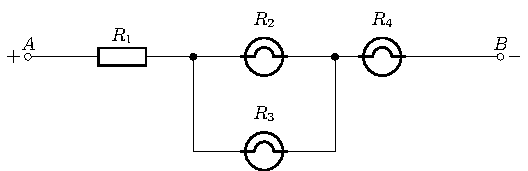
\includegraphics{fig/B/7-21.pdf}
        \caption{}\label{fig_B_7-21}
    \end{figure}

    \item 图~\ref{fig_B_7-22} 中,电源电压为220伏,各段输电导线上的电阻$r$都为2欧,用电器$R_1$的电阻为200欧,$R_2$的电阻为196欧.
    $R_1$、$R_2$两端的电压各是多少?
    \begin{figure}[htbp]
        \centering
        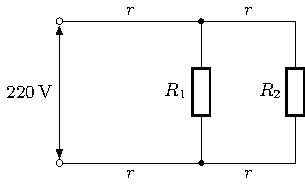
\includegraphics{fig/B/7-22.pdf}
        \caption{}\label{fig_B_7-22}
    \end{figure}

    \item 一个600欧的电阻和一个400欧的电阻串联后接在电压为90伏的电源上.
    用伏特表测得600欧电阻上的电压为45伏.
    \begin{enumerate}
        \item 伏特表接入电路后,600欧电阻上的电压改变了多少?
        \item 这个伏特表的内阻是多少?
    \end{enumerate}
    \item 在图~\ref{fig_B_7-23} 中滑动变阻器作分压器使用.
    负载电阻$R$一端接在变阻器的固定端$A$上,另一端接在滑动端$P$上.
    滑动端$P$在$AB$间移动时,$R$上就能得到不同的电压.
    \begin{enumerate}
        \item 当滑动端从$A$向$B$移动时,$R$上的电压怎样变化?
        \item 如果电压$U=6 \UV$,变阻器的电阻$R_{AB}=50\UO$,负载电阻$R=100\UO$.
        当滑动端$P$在$A$点、$B$点时,$R$上的电压各是多少?
        \item 当$P$在$AB$中点时,$R$上的电压是否为3伏?通过变阻器各部分的电流是否相等?
    \end{enumerate}
    \begin{figure}[htbp]
    	\centering
    	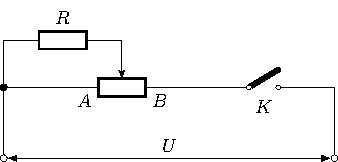
\includegraphics{fig/B/7-23.pdf}
    	\caption{}\label{fig_B_7-23}
    \end{figure}
\end{enumerate}

\section{电动势~~闭合电路的欧姆定律}

要使电路中有电流,必须把电路与电源相连,组成闭合电
路.闭合电路中的电流强度跟什么有关系呢?为了研究这个问题,需要先介绍一个表征电源特性的物理量——电动势.

\subsection{电动势}


电源有两个极,正极的电势比负极的高,两极间有一定的电压.电源的作用就是保持两极间有一定的电压.把伏特表接在干电池的正、负极上(图~\ref{fig_B_7-24}),可以测得干电池两极间的电压是1.5伏.用伏特表对不同型号的干电池进行测量,结果表明,它们两极间的电压都是1.5伏.用伏特表测量蓄电池两极间的电压,结果表明,只要蓄电池是同种的,它们两极间的电压都相同,例如常用的铅蓄电池两极间的电压是2伏.可见,同种电源两极间的电压相同,不同种类的电源,一般说来,两极间的电压不相同.为了表征电源的这种特性,物理学中引入了电动势这个物理量.电源的电动势在数
值上等于电源没有接入外电路时两极间的电压,上面把伏特表直接接在电源的两极上测出的就是电源的电动势.

\begin{figure}[htbp]
	\centering
	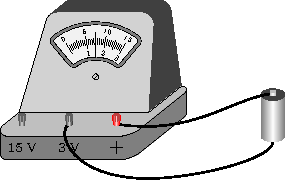
\includegraphics{fig/B/7-24.pdf}
	\caption{}\label{fig_B_7-24}
\end{figure}


把电源跟外电路接通后,再用伏特表测量两极间的电压
(图~\ref{fig_B_7-25}),可以看到,这时伏特表的读数小于电源的电动势.这是什么原因呢?原来,在电源跟外电路接通后,不仅外电路中有电流通过,电源内部的电路中也有电流通过.内电路也有电阻,所以电流通过内电路时也产生电势降落.电源的电动势是一定的,要不是内电路中也有电势降落,接通电路后外电路两端的电压应该等于电源的电动势.考虑到内电路上的电势降落,我们可以设想内、外电路上的电势降落之和应该等于电源的电动势.
\begin{figure}[htbp]
    \centering
    \begin{minipage}[t]{0.4\textwidth}
        \centering
        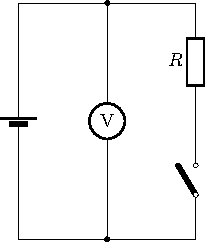
\includegraphics{fig/B/7-25.pdf}
        \caption{}\label{fig_B_7-25}
    \end{minipage}
    \hfil
    \begin{minipage}[t]{0.53\textwidth}
        \centering
        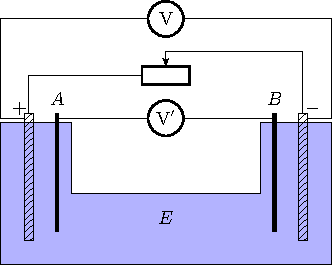
\includegraphics{fig/B/7-26.pdf}
        \caption{内、外电路上的电压之和等于电动势}\label{fig_B_7-26}
    \end{minipage}
\end{figure}

实际情况是否如此呢?这需要用实验来验证.
在图~\ref{fig_B_7-26} 中,$E$是实验用的电池,滑动变阻器作外电路;伏特表$V$连接在电池的两极上,用来测量外电路上的电压$U$;伏特表$V'$连接在插在电极附近的探针$A$和$B$上,用来测量内电路上的电压$U'$.先断开外电路,用伏特表$V$测出电源的电动势$\mathcal{E}$.然后接通外电路,测量$U$和$U'$.移动变阻器的滑动头,改变外电路的电阻,从而改变电路中的电流强度,可以看到,内、外电路上的电压$U$和$U'$也随着变化,但是$U$和$U'$之和却保持不变.总等于电源的电动势$\mathcal{E}$.
即
\[\mathcal{E}=U+U'\]
这表明,在外电路接通时,电源的电动势等于内、外电路上的电压之和.

利用这个结果,我们可以从电路中能量转化的角度来理
解电动势的物理意义.在公式$\mathcal{E}=U+U'$中,右端$U+U'$在数值上等于1库仑电量通过外电路和内电路时消耗的总电能.电路中消耗的电能是由电源提供的,公式左端的$\mathcal{E}$在数值上等于电路中通过$1$库仑电量时电源提供的能量.因此,\NoteUnderWave{电动势反映了电源的一种特性,它在数值上等于电路中通过1库仑电量时电源所提供的电能}.电源提供的电能是由其他形式的能转化来的.例如,在化学电池中电能是由化学能转化来的,在发电机中电能是由机械能转化来的.从本质上来说,各种电源都是把其他形式的能转化为电能的装置.电动势越大,表明电源把其他形式的能转化为电能的本领越大.

\subsection{闭合电路的欧姆定律}

利用前面得出的公式$\mathcal{E}=U+U'$和欧姆定律,就可以求出闭合电路中的电流强度跟什么有关
系.如果用$R$表示外电路的电阻,$r$表示内电路的电阻,$I$表示电路中的电流强度,那么,根据欧姆定律可以写出:$U=IR$,$U'=Ir$,代入$\mathcal{E}=U+U'$中,可得
\[\mathcal{E}=IR+Ir \]
由此可得
\[I=\frac{\mathcal{E}}{R+r} \]

这就是\NoteBold{闭合电路的欧姆定律}.它表示:\NoteBold{闭合电路中的电流强度跟电源的电动势成正比,跟内、外电路中的电阻之和成反比}.

这是关于电路的一条重要定律,以后经常要用到.

\begin{example}
在图~\ref{fig_B_7-27} 中,$R_1=14.0 \UO$,$R_2=9.0 \UO$.
当单刀双掷开关$K$扳到位置1时,测得电流强度$I_1=0.20\UA $;当$K$扳到位置2时,测得电流强度$I_2=0.30\UA $.求电源的电动势和内电阻.
\end{example}
\begin{figure}[htbp]
    \centering
    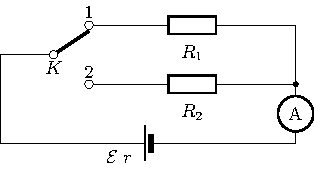
\includegraphics{fig/B/7-27.pdf}
    \caption{}\label{fig_B_7-27}
\end{figure}

\begin{solution}
    根据闭合电路的欧姆定律,可列出方程组:
    \[\begin{split}
        \mathcal{E}&=I_1R_1+I_1r\\
        \mathcal{E}&=I_2R_2+I_2r\\
    \end{split}\]
    消去$\mathcal{E}$,可得
    \[I_1 R_1+I_1r=I_2R_2+I_2r\]
    所以,电源的内电阻
\[\begin{split}
    r&=\frac{I_1R_1-I_2R_2}{I_2-I_1}\\
    &=\frac{0.20\times 14.0-0.30\times 9.0}{0.30-0.20} \UO =1.0\UO
\end{split}\]
    把$r$值代入$\mathcal{E}=I_1R_1+I_1r$中,可得电源的电动势
    \[\mathcal{E}=(0.20\times 14.0 +0.20\times 1.0) \UV =3.0 \UV \]
\end{solution}

这道例题介绍了一种测量电源的电动势和内电阻的方法.


\section*{阅读材料:欧姆定律的建立}

欧姆是德国物理学家,当过多年的中学数学和物理教师,对研究工作很有雄心抱负.他在缺少时间和书籍以及适当的仪器的情况下,自己制作了许多仪器,独自坚持研究工作.经过多年努力,终于建立了欧姆定律.

在欧姆进行研究时,科学上还没有建立起电动势、电流强度、电阻等明确的概念,更没有准确测量这些量的仪器.欧姆进行实验时所用的电源是温差电偶,他用验电器测量电源两端的电势差.欧姆用许多粗细相同、长度不同的铜导线作为电阻进行实验,他根据电流使悬挂的磁针偏转的角度来测量电流的强弱.1826年欧姆根据测得的数据得出了下面的公式
\[\chi=\frac{a}{b+x}\]

其中$\chi$代表电流磁效应的强弱,相当于电流强度;$x$代表铜导线的长度,相当于电阻;$a$代表电源的“激活力”,也就是电动势;$b$由电路其他部分决定,如果不考虑连接导线的影响,则相当于电源的内电阻.上式相当于课文中讲的全电路欧姆定律的公式.

在实验研究的基础上,欧姆把电流跟热流、水流等现象进行对比,从中得到启发,认为电流中的电势差起着跟热流中的
温度差、水流中的高度差相似的作用.通过对比,他引入了电流强度、电动势、电阻等概念,并确定了它们之间的关系.


\subsection*{练习八}
\begin{enumerate}
    \item 电源的电动势为1.5伏,内电阻为0.12欧,外电路的电阻为1.28欧,求电路中的电流强度.
    \item 把一个定值电阻和电源连成图~\ref{fig_B_7-28} 所示的电路,可以测得电源的内电阻.
    定值电阻$R$为10欧,合上开关$K$时,伏特表的读数为5.46伏.
    打开$K$时,伏特表的读数为6.0伏.求电源的内电阻为多少.
    \begin{figure}[htbp]
        \centering
        \begin{minipage}[t]{0.48\textwidth}
            \centering
            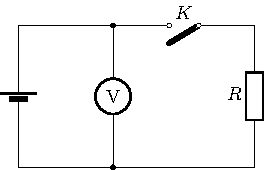
\includegraphics{fig/B/7-28.pdf}
            \caption{}\label{fig_B_7-28}
        \end{minipage}
        \begin{minipage}[t]{0.48\textwidth}
            \centering
            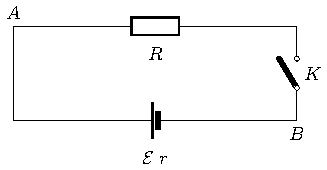
\includegraphics{fig/B/7-29.pdf}
            \caption{}\label{fig_B_7-29}
        \end{minipage}
    \end{figure}
    \item 在图~\ref{fig_B_7-29} 所示的电路中$\mathcal{E}=9.0 \UV$,$r=3.0 \UO$,$R=15 \UO$,当$K$闭合时,$U_{AB}$是多少?当$K$打开时,$U_{AB}$又为多少?
    \item 利用图~\ref{fig_B_7-30} 所示的电路可以测出电源的电动势和内电阻.当变阻器的滑动端在某一位置时,安培表和伏特表的读数分别是0.20安和1.98伏.
    改变滑动端的位置后,两表的读数分别是0.40安和1.96伏.
    求电池的电动势和内电阻.
    \begin{figure}[htbp]
        \centering
        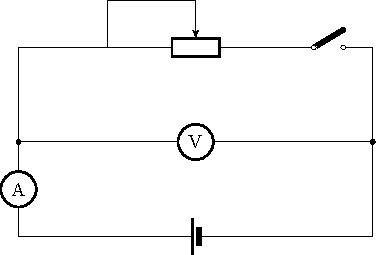
\includegraphics{fig/B/7-30.pdf}
        \caption{}\label{fig_B_7-30}
    \end{figure}
\end{enumerate}




  

\section{路端电压}
从图~\ref{fig_B_7-26} 所示的实验中可以看出,外电路中的电阻发生变化时,内、外电路上的电压$U'$和$U$都随着变化.因为用电器都是接在外电路中的,电源的“有效”电压是外电路上的电压,因此,研究外电路上的电压的变化规律是很重要的.
通常把外电路两端的电压叫做\NoteBold{路端电压}.下面我们用闭合电路的欧姆定律来分析路端电压的变化规律.

公式$\mathcal{E}=U+U'$可以改写作$U=\mathcal{E}-U'$,这表示路端电压
等于电源的电动势减去电源内部的电压.因为$U'=Ir$,代入式中可得
\[U=\mathcal{E}-Ir\]

就某个电源来说,电动势$\mathcal{E}$和内电阻$r$都是一定的,从上式可以看出路端电压$U$跟电路中的电流强度有关系.电流强度$I$增大时,电源内部的电压$Ir$增大,路端电压就减小;电流强度减小时,电源内部的电压$Ir$减小,路端电压就增大.路端电压所以随电流而变化,根本原因是电源有内电阻,如果没有内电阻,不论电流怎样变化,路端电压也不会变化,总等于电源的电动势.


路端电压跟电流强度的关系常用图线来表示,用横轴表示电流强度$I$,纵轴表示路端电压$U$,利用上面的关系式可以画出$U-I$关系曲线(图~\ref{fig_B_7-31}).从图上可以看出,此关系曲线
是一条向下倾斜的直线.当$I=0$时,$U=\mathcal{E}$;随着$I$的增大,$U$逐渐减小,直线倾斜的程度跟内电阻有关系,内电阻越大,倾斜得越厉害;内电阻越小,这条直线越平;内电阻趋于零时,这条直线趋近于跟横轴平行.

\begin{figure}[htbp]
	\centering
	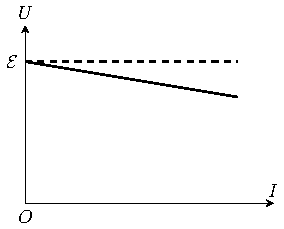
\includegraphics{fig/B/7-31.pdf}
	\caption{$U-I$关系曲线}\label{fig_B_7-31}
\end{figure}



根据闭合电路的欧姆定律,电流强度$I=\mathcal{E}/(R+r)$.$\mathcal{E}$和$r$都是不变的,电流强度$I$是随外电阻$R$而变化的,因此,路端电压也随外电阻$R$而变化.$R$增大时,$I$减小,路端电压增大;$R$减小时,$I$增大,路端电压减小.

下面来讨论两种特殊情况.

(1)当外电路断开,即断路时,$R$变成无限大,$I$变为零,$Ir$也变为零,$U$等于$\mathcal{E}$,即断路时的路端电压等于电源的电动势.

上一节我们讲过,用伏特表测出的断路时的路端电压就
是电源的电动势.可是这时伏特表本身成了外电路,因此测出的路端电压并不准确地等于电动势,不过由于伏特表的电阻很大,电路中的电流很小,
$Ir$也很小,因此$U$和$\mathcal{E}$相差很小.只要不要求特别准确,用这个办法测电动势很方便.

(2)当$R$趋近于零,即短路时,路端电压$U$也趋近于零,这时电流强度就趋近于$\mathcal{E}/r$.

发生短路时,电流强度取决于电源的电动势和内电阻.电源的内电阻一般都很小,例如铅蓄电池的内电阻只有0.005—0.1欧姆,所以短路时电流很大.这时电源提供的全部能量都消耗在内电路上,短时间内将产生很大的热量,会烧毁电源.因此在实际中要切实注意防止短路.

\subsection*{练习九}

\begin{enumerate}
    \item 试分析说明:外电路中的电阻发生变化时为什么会影响路端电压的变化.
    \item 在两个电路中,电源的电动势相同,但内电阻不同,当它们的外电路中流过的电流相同时,哪个电路的路端电压大?
    \item 在图~\ref{fig_B_7-32} 所示的电路中,当$P$由左向右滑动时,安培表和伏特表的读数怎样变化?$P$的位置在何处,伏特表的
指示更接近于电源的电动势?

\begin{figure}[htbp]
    \centering
    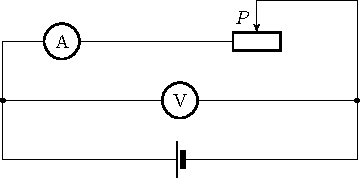
\includegraphics{fig/B/7-32.pdf}
    \caption{}\label{fig_B_7-32}
\end{figure}

\item 发电机的电动势为240伏,内电阻为0.40欧,给200盏电阻均为1210欧的电灯供电,电灯上的电压是多大?如果
再接入100盏同样的电灯,电灯上的电压又是多大?利用所得的结果说明:电路中的用电器增多时,加在用电器上的电压将
怎样变化?
\end{enumerate}


\section{电池组}
我们知道,用电器要在额定电压和额定电流下才能正常工作.任何一个电池都有一定的电动势和允许通过的最大电流.如果用电器的额定电压低于电池的电动势,额定电流也小于电池允许通过的最大电流,我们可以用单个电池来给电路供电.实际上,用电器的额定电压常常高于电池的电动势,
额定电流也常常大于电池允许通过的最大电流,在这种情况下,需要把几个电池连成电池组,以便提高供电的电压或者增大输出的电流.晶体管收音机的直流电源,火车上照明用的电源,汽车发动机启动和照明用的电源,都是用电池组.电池组一般都是用相同的电池组成的.

\subsection{串联电池组}

把第一个电池的负极和第二个电池的正极
相连接,再把第二个电池的负极和第三个电池的正极相连接,像这样依次连接起来,就组成了串联电池组(图~\ref{fig_B_7-33}).第一个电池的正极就是电池组的正极,最后一个电池的负极就是电池组的负极.
\begin{figure}[htbp]
    \centering
    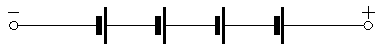
\includegraphics{fig/B/7-33.pdf}
    \caption{}\label{fig_B_7-33}
\end{figure}

设串联电池组是由$n$个电动势都是$\mathcal{E}$、内电阻都是$r$的电池组成.由于开路时路端电压等于电源的电动势,每一个电池正极的电势比它负极的电势高$\mathcal{E}$,而前一个电池的负极和后一个电池的正极电势相同.因此,串联电池组正极的电势比
它负极的电势高$n\mathcal{E}$.
整个电池组的电动势
\[\mathcal{E}_{\text{串}}=n\mathcal{E}\]
电池是串联的,电池的内电阻也是串联的,串联电池组的内电阻
\[r_{\text{串}}=nr\]

\NoteUnderWave{串联电池组的电动势等于各个电池电动势之和,串联电池组的内电阻等于各个电池内电阻之和.}

串联电池组的电动势比单个电池的高,当用电器的额定
电压高于单个电池的电动势时,可以用串联电池组供电.这时全部电流要通过每个电池,用电器的额定电流必须小于单
个电池允许通过的最大电流.

把几个电池组成串联电池组时,注意不要把某些电池接反.例如,用两个1.5伏特电池组成串联电池组,如果连接正确,可以得到3伏特的电动势,使小灯泡发光(图~\ref{fig_B_7-34a});如果接反了,则电池组的电动势为零,小灯泡不发光(图~\ref{fig_B_7-34b}).
\begin{figure}[htbp]
    \centering
    \begin{subfigure}{0.4\linewidth}
        \centering
        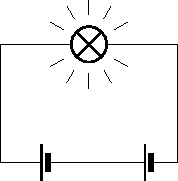
\includegraphics{fig/B/7-34a.pdf}
        \caption{}\label{fig_B_7-34a}
    \end{subfigure}
    \hfil
    \begin{subfigure}{0.4\linewidth}
        \centering
        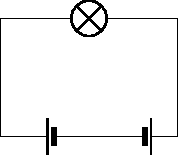
\includegraphics{fig/B/7-34b.pdf}
        \caption{}\label{fig_B_7-34b}
    \end{subfigure}
    \caption{}\label{fig_B_7-34}
\end{figure}



\subsection{并联电池组}


把电动势相同的电池,正极和正极相连接,负极和负极相连接,就组成并联电池组(图~\ref{fig_B_7-35}).连在一起的正极是电池组的正极,连在一起的负极是电池组的负极.
\begin{figure}[htbp]
    \centering
    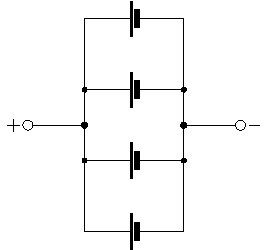
\includegraphics{fig/B/7-35.pdf}
    \caption{}\label{fig_B_7-35}
\end{figure}

设并联电池组是由$n$个电动势都是$\mathcal{E}$、内电阻都是$r$的电池组成的.用导线连接起来的所有极板的电势都相等,所以并联电池组正负极间的电势差等于每个电池正负极间的电势差.而开路时正负极间的电势差等于电动势,所以并联电池组的电动势
\[\mathcal{E}_{\text{并}}=\mathcal{E} \]
电池是并联的,电池的内电阻也是并联的,并联电池组的内电阻
\[r_{\text{并}}=\frac{r}{n} \]

\NoteUnderWave{由$n$个电动势和内电阻都相同的电池连成的并联电池组,它的电动势等于一个电池的电动势,它的内电阻等于一个电池的内电阻的$n$分之一}.

并联电池组的电动势虽然不高于单个电池的电动势,但每个电池中通过的电流只是全部电流的一部分,整个电池组允许通过较强的电流.因此,用电器的额定电流比单个电池允许通过的最大电流大时,可以采用并联电池组供电.

当电池的电动势和允许通过的最大电流都小于用电器的额定电压和额定电流时,可以先组成几个串联电池组,再把几个串联电池组并联起来,使用电器得到所需的电压,而且每个电池实际通过的电流小于允许通过的最大电流.像这样把几个串联电池组再并联起来组成的电池组,叫做混联电池组.


\subsection*{练习十}
\begin{enumerate}
    \item 每个铅蓄电池的电动势为2.0伏,想用它们给一个额定电压为6伏的用电器供电,应该怎么办?
    \item 每节干电池的电动势为1.5伏,允许通过的最大电流为0.05安.现在需要一个电动势为6伏,最大电流为0.1安的电源,应该怎么办?
    \item 有10个相同的蓄电池,每个蓄电池的电动势为2.0伏,内电阻为0.04欧.
    把这些蓄电池接成串联电池组,外接电阻为3.6欧.求电路中的电流强度和电池组两端的电压.
    \item 找一个半导体收音机,打开看看里面有几节干电池,是怎样连接的,算一算这个收音机的电源电压是多少.
    \item 把两节干电池串联起来组成电池组,用伏特表量出电池组的电动势.再把三个小灯泡照图~\ref{fig_B_7-36} 依次连入电路中,注意每增加一个小灯泡时伏特表读数的变化.
    说明伏特表的读数为什么会发生变化.这个变化表明了什么?
\end{enumerate}

\begin{figure}[htbp]
    \centering
    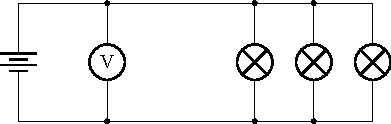
\includegraphics{fig/B/7-36.pdf}
    \caption{}\label{fig_B_7-36}
\end{figure}


\section{电阻的测量}
我们在实际工作中经常需要测量电阻.测量电阻的方法很多,我们先讨论原理最简单的伏安法,然后介绍实际测量中常用的欧姆表和惠斯通电桥.

\subsection{伏安法}

根据欧姆定律$U=IR$,用伏特表测出电阻两端的电压,用安培表测出通过电阻的电流,就可以求出电阻值,这就是测量电阻的伏安法.

伏安法测量电阻在原理上是非常简单的,但由于伏特表
和安培表都有内阻,把它们连入电路中不可避免地要改变电路本身,这就给测量结果带来了误差.
\begin{figure}[htbp]
    \centering
    \begin{subfigure}{0.4\linewidth}
        \centering
        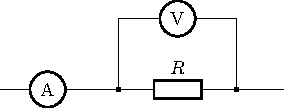
\includegraphics{fig/B/7-37a.pdf}
        \caption{}\label{fig_B_7-37a}
    \end{subfigure}
    \hfil
    \begin{subfigure}{0.4\linewidth}
        \centering
        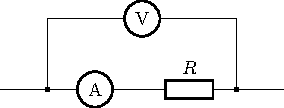
\includegraphics{fig/B/7-37b.pdf}
        \caption{}\label{fig_B_7-37b}
    \end{subfigure}
    \caption{}\label{fig_B_7-37}
\end{figure}

用伏安法来测电阻,可以有两种方法把伏特表和安培表连入电路,如图~\ref{fig_B_7-37} 所示.采用图~\ref{fig_B_7-37a} 的接法时,由于
伏特表的分流,安培表测出的电流强度比通过电阻的电流强度要大些,这样计算出的电阻值就要比真实值小些.
采用图~\ref{fig_B_7-37b} 的接法时,由于安培表的分压,伏特表测出的电压比电阻两端的电压大些,这样计算出的电阻值就要比真实值大些.

待测电阻的阻值比伏特表的电阻值小得越多,采用图~\ref{fig_B_7-37a} 的接法时由于伏特表的分流而引起的误差越小.因此,测量小电阻时应采用这种接法.

待测电阻的阻值比安培表的电阻值大得越多,采用图~\ref{fig_B_7-37b} 的接法时由于安培表的分压而引起的误差越小.
因此,测量大电阻时应采用这种接法.

\subsection{欧姆表}


伏安法测电阻比较麻烦,实际中常用能直接读出电阻值的欧姆表来测电阻.

欧姆表是根据闭合电路的欧姆定律制成的,它的原理如图~\ref{fig_B_7-38} 所示.$G$是内阻为$R_g$、满度电流为$I_g$的电流表.$R$是可变电阻,也叫调零电阻.电池的电动势是$\mathcal{E}$、内电阻是$r$.

\begin{figure}[htbp]
	\centering
	\begin{subfigure}{0.3\linewidth}
		\centering
		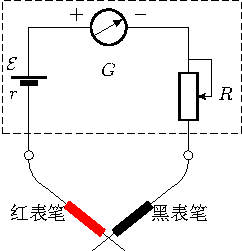
\includegraphics{fig/B/7-38a.pdf}
		\caption{}\label{fig_B_7-38a}
	\end{subfigure}
	\hfil
	\begin{subfigure}{0.3\linewidth}
		\centering
		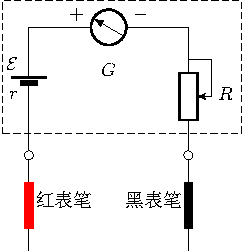
\includegraphics{fig/B/7-38b.pdf}
		\caption{}\label{fig_B_7-38b}
	\end{subfigure}
	\hfil
	\begin{subfigure}{0.3\linewidth}
		\centering
		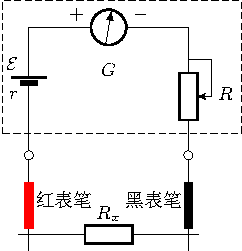
\includegraphics{fig/B/7-38c.pdf}
		\caption{}\label{fig_B_7-38c}
	\end{subfigure}
	\caption{}\label{fig_B_7-38}
\end{figure}




当红、黑表笔相接时(图~\ref{fig_B_7-38a}),调节$R$的阻值,使
\[\frac{\mathcal{E}}{R_g+r+R}=I_g\]
则指针指到满刻度,表明红、黑表笔间的电阻
为零.当红、黑表笔不接触时(图~\ref{fig_B_7-38b}),电路中没有电流,指针不偏转,即指着电流表的零点,表明表笔间的电阻是无限大.当红、黑表笔间接入某一电阻$R_x$时(图~\ref{fig_B_7-38c}),则通
过电流表的电流强度
\[I=\frac{\mathcal{E}}{R_g+r+R+R_x}\]
$R_x$改变,$I$随着改
变,每一个$R_x$值都有一个对应的电流强度值$I$.如果在刻度盘上直接标出与$I$对应的电阻值$R_x$,用红、黑表笔分别接触待测电阻的两端,就可以从表盘上直接读出它的阻值.

用欧姆表测电阻是很方便的,但是电池用久了,它的电动
势和内电阻都要变化,那时欧姆表指示的电阻值,误差就相当大了.所以欧姆表只能用来粗略地测量电阻.



\section{惠斯通电桥$^\star$}
用欧姆表测量电阻虽然很方便,但不够准确.在实验室里要比较准确地测量电阻,常用惠斯通电桥.


图~\ref{fig_B_7-39} 是惠斯通电桥的
电路图.四个电阻$R_1$、$R_2$、$R_3$、$R_x$连成四边形,每一边叫做电桥的一个臂.$R_x$是待测电阻,其余三个是可调的已知电阻.电源接在$A$、$C$两点之间.
灵敏电流表$G$接在$B$、$D$两点之间,用来比较这两点的电势是否相等.所谓“桥”指的就是$B$、$D$两点间的连线.当$B$、$D$两点的电势相等时,叫做\NoteBold{电桥平衡},这时通过电流表$G$的电流强度$I_g=0$.当$B$、$D$两点的电势不相等时,叫做电桥不平衡,这时有电流通过电流表.

\begin{figure}[htbp]
	\centering
	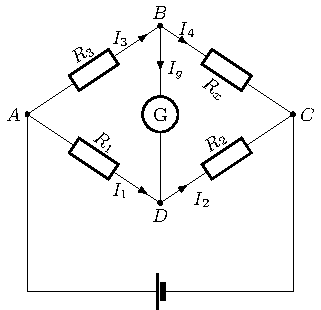
\includegraphics{fig/B/7-39.pdf}
	\caption{}\label{fig_B_7-39}
\end{figure}

惠斯通电桥是利用电桥平衡条件来测量电阻的.测量
时,调节电阻$R_1$、$R_2$、$R_3$的阻值,使通过电流表的电流强度$I_g=0$.这时电桥平衡,表明$B$、$D$两点的电势相等.所以
\[\begin{split}
    U_{AB}&=U_{AD}\\
    U_{BC}&=U_{DC}
\end{split}\]
$U_{AB}=I_3R_3$,$U_{AD}=I_1R_1$,$U_{BC}=I_4R_x$, $U_{DC}=I_2R_2$.代入上面二式中,可得
\[\begin{split}
    I_3R_3&=I_1R_1\\
I_4R_x&=I_2R_2
\end{split}\]

因为这时通过电流表的电流强度$I_g=0$,所以通过$AB$和$BC$ 两臂的电流强度相等,即$I_3=I_4$,通过$AD$和$DC$两臂的电流强度也相等,即$I_1=I_2$.代入上面二式中,并把二式相除,最后得到
\[\frac{R_3}{R_x}=\frac{R_1}{R_2} \]
或\[R_x=\frac{R_2R_3}{R_1} \]

把已知的$R_1$、$R_2$、$R_3$的阻值代入,即可求出待测电阻$R_x$的值.

用惠斯通电桥测量电阻,精确度跟已知电阻的准确程度
和电流表的灵敏度有关.因为在测量时我们是根据电流表指针是否偏转来判断电桥是否平衡的,电流表不偏转,并不说明通过电流表的电流强度$I_g$绝对为零,只是说明$I_g$小到电流表检测不出来的程度.所以,已知电阻的准确程度越高,电流表的灵敏度越高,我们的测量结果就越精确.

惠斯通电桥有多种形式,学校里常用的是滑线式电桥,如图~\ref{fig_B_7-40} 所示.电桥的主要部分是一条1米长的均匀的电阻线$AC$.待测电阻$R_x$接在$B$、$C$间,作已知电阻用的电阻箱$R$接在$A$、$B$间.$D$是滑动触头,可沿$AC$线移动,平时不跟$AC$线接触,按下后接通,松手后又断开.

\begin{figure}[htbp]
    \centering
    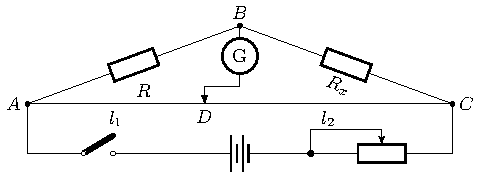
\includegraphics{fig/B/7-40.pdf}
    \caption{}\label{fig_B_7-40}
\end{figure}

电阻线$AC$是均匀的,$AD$段的电阻跟$DC$段的电阻之比等于它们的长度比$\ell_1/\ell_2$.接通电路,按下触头后,如果电流表中没有电流通过,我们可以用
\[R_x=\frac{\ell_2}{\ell_1}R\]
算出$R_x$的阻值.

\subsection*{练习十一}
\begin{enumerate}
    \item 在图~\ref{fig_B_7-37a} 中,如果安培表的读数是0.2安,伏特表的读数是30伏,根据这些数据算出的$R$的阻值是多大?如果已知伏特表的内阻是3千欧,那么,$R$的真实值是多大?采用这种接法时,算出的$R$值比真实值大还是小?
    \item 在图~\ref{fig_B_7-37b} 中,如果伏特表的读数是5伏,安培表的读数是0.5安,根据这些数据算出的$R$的阻值是多大?如果已知安培表的内阻是0.2欧,那么,$R$的真实值是多大?采用这种接法时,算出的$R$值比真实值大还是小?
    \item 已知伏特表的内阻为5千欧,安培表的内阻为0.2欧.
    如果用它们来测量一个线圈的电阻,估计这个线圈的电阻大约为几个欧姆,那么,怎样连接电路测得的结果误差较小?画出电路图.
    \item$^\star$ 在图~\ref{fig_B_7-40} 中,$R$为15欧,电桥平衡时,$\ell_1$为0.45米,$\ell_2$为0.55米,求待测电阻$R_x$.
    \item$^\star$ 在图~\ref{fig_B_7-40} 中,如果$AB$支路发生断路,当滑动触头
    $D$从$A$移向$C$时,电流表$G$中的电流如何变化?如果$BC$支路发生断路,当$D$从$A$移向$C$时,电流表$G$中的电流又如何变化?
\end{enumerate}

\section*{复习题}
\begin{enumerate}
    \item 什么是电流?什么是电流强度?存在持续电流的条件是什么?金属导体中的电流是怎样形成的?
    \item 欧姆定律的内容和公式是什么?
    \item 电阻定律的内容和公式是什么?什么是材料的电阻率?
    \item 写出电功和电功率的公式.
    在电路中,电流做功消耗了什么能?消耗的能量是由什么供给的?
    \item 什么是用电器的额定电压和额定功率?当加在用电
    器上的电压低于额定电压时,用电器的实际功率还等于额定功率吗?
    \item 串联电路中电流、电压的基本特点是什么?串联电路的总电阻、电压分配和功率分配是怎样的?为什么串联电阻有分压作用?
    \item 并联电路中电流、电压的基本特点是什么?并联电路的总电阻、电流分配和功率分配是怎样的?为什么并联电阻有分流作用?
    \item 把电流表改装为安培表应该串联还是并联一个电阻?为什么?改装为伏特表呢?
    \item 电源的电动势等于什么?闭合电路的欧姆定律的内容和公式是什么?
\item 什么是路端电压?外电路上的电阻增大或减小时,路端电圧怎样变化?为什么这样变化?
\item 串联电池组的电动势和内电阻各等于什么?并联电池组呢?在什么情况下应使用串联电池组?在什么请况下应使用并联电池组?
\item 伏安法测电阻的原理是什么?试分析说明伏安法测电阻产生误差的原因.
\item 说明欧姆表的原理.
\item$^\star$ 惠斯通电桥测量电阻的原理是什么?
\end{enumerate}


\section*{习题}



\begin{enumerate}
    \item 在图~\ref{fig_B_7-41} 中,电键可以向左扳将$a$与1接通,也可以向右扳将$a$与2接通.
    电键接通1的瞬间,电流的方向怎样?
接通1后再向右扳电键,将$a$与2接通,接通2的瞬间,电流的方向又怎样?
\begin{figure}[htbp]
	\centering
	\begin{minipage}[t]{0.48\textwidth}
		\centering
		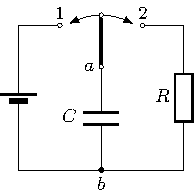
\includegraphics{fig/B/7-41.pdf}
		\caption{}\label{fig_B_7-41}
	\end{minipage}
	\begin{minipage}[t]{0.48\textwidth}
		\centering
		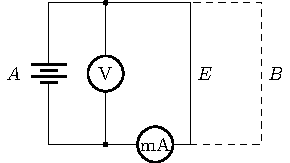
\includegraphics{fig/B/7-42.pdf}
		\caption{}\label{fig_B_7-42}
	\end{minipage}
\end{figure}
\item $A$和$B$两地相距40千米,从$A$到$B$的两条输电线的总电阻为800欧,如果在$A$、$B$之间的某处$E$两条电线发生短路(图~\ref{fig_B_7-42}),可用伏特表、毫安表和电池组检查出发生短路的地点.如果在$A$处测得伏特表的读数是10伏,毫安表的读数是40毫安.
求短路处$E$到$A$的距离.
\item 有两个灯泡,一个是110伏、100瓦,一个是110伏、
40瓦,把它们串联后接入220伏的电路中使用行不行?为什么?有一个变阻器,把它怎样连入电路中可以使两灯泡正常发光?这时变阻器的阻值应调至多大?
\item 有一用电器$W$,额定电压为100伏,额定功率为150瓦.
用120伏的电源供电.为了使用电器能正常工作,用一
电阻为210欧的变阻器进行分压(图~\ref{fig_B_7-43}).$R_1$、$R_2$为多大时,用电器才能正常工作?
\begin{figure}[htbp]
	\centering
	\begin{minipage}[t]{0.48\textwidth}
		\centering
		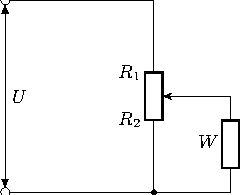
\includegraphics{fig/B/7-43.pdf}
		\caption{}\label{fig_B_7-43}
	\end{minipage}
	\begin{minipage}[t]{0.48\textwidth}
		\centering
		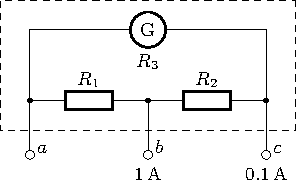
\includegraphics{fig/B/7-44.pdf}
		\caption{}\label{fig_B_7-44}
	\end{minipage}
\end{figure}
\item 图~\ref{fig_B_7-44} 所示的是有两个量程的安培表,当使用$a$、$b$两端点时,量程为1安,当使用$a$、$c$两端点时,量程为0.1安.已知电流表的内阻$R_g$为200欧,满度电流$I_g$为2毫安,求电阻$R_1$和$R_2$.

\item 在图~\ref{fig_B_7-27} 中,不用安培表,改用伏特表能不能测出电源的电动势和内电阻?画出伏特表应怎祥接入电路,说明要取得哪些数据,写出计算电动势和内电阻的公式.
\item 在图~\ref{fig_B_7-45} 中,用一台直流发电机$F$给一台电动机$M$和一些电灯供电.已知发电机的电动势$\mathcal{E}=240 \UV $,内电阻$r=1 \UO $,输电线的总电阻$R=3 \UO $,电动机的工作电流为3安,供给电灯的总电流为9安.
求电灯和电动机两端的电压.
\begin{figure}[htbp]
    \centering
    \includegraphics{fig/B/7-45.pdf}
    \caption{}\label{fig_B_7-45}
\end{figure}

\item 现有电动势为1.5伏,内电阻为1欧的电池若干,每个电池允许输出的电流为0.05安,又有不同阻值的电阻可作为分压电阻.
试设计一种电路,使额定电压为6伏、额定电流为0.1安的用电器正常工作.
画出电路图,并标明分压电阻的值.
\item 用伏安法测电阻,如果所用的安培表的内阻$R_A=0.1 \UO $
,伏特表的内阻$R_V=1000 \UO $,那么,用图~\ref{fig_B_7-37} 所示的两种不同接法测量$R=1 \UO $的电阻时,哪种方法产生的误差较小?测量$R=500 \UO $的电阻时,哪种方法产生的误差较小?测量较小的电阻和较大的电阻,各应采用什么方法?
\item$^\star$ 在图~\ref{fig_B_7-40} 中,滑动触头$D$从$A$向$C$移动时,电流
表中都有电流通过,但电流强度逐渐减小,这时可能是什么地方发生了断路?如果电流表指示的电流强度逐渐增大,又可能是什么地方发生了断路?
\item$^\star$ 在图~\ref{fig_B_7-40} 中,无论在从$A$经电源到$C$的电路中发
生断路,还是从$B$经电流表到$D$的电路中发生断路,在按下滑动触头时都没有电流通过电流表.用什么办法可以把这两种情况区别开来?
\end{enumerate}






